\section{Схема установки}

\begin{figure}[h!]
	\begin{center}
		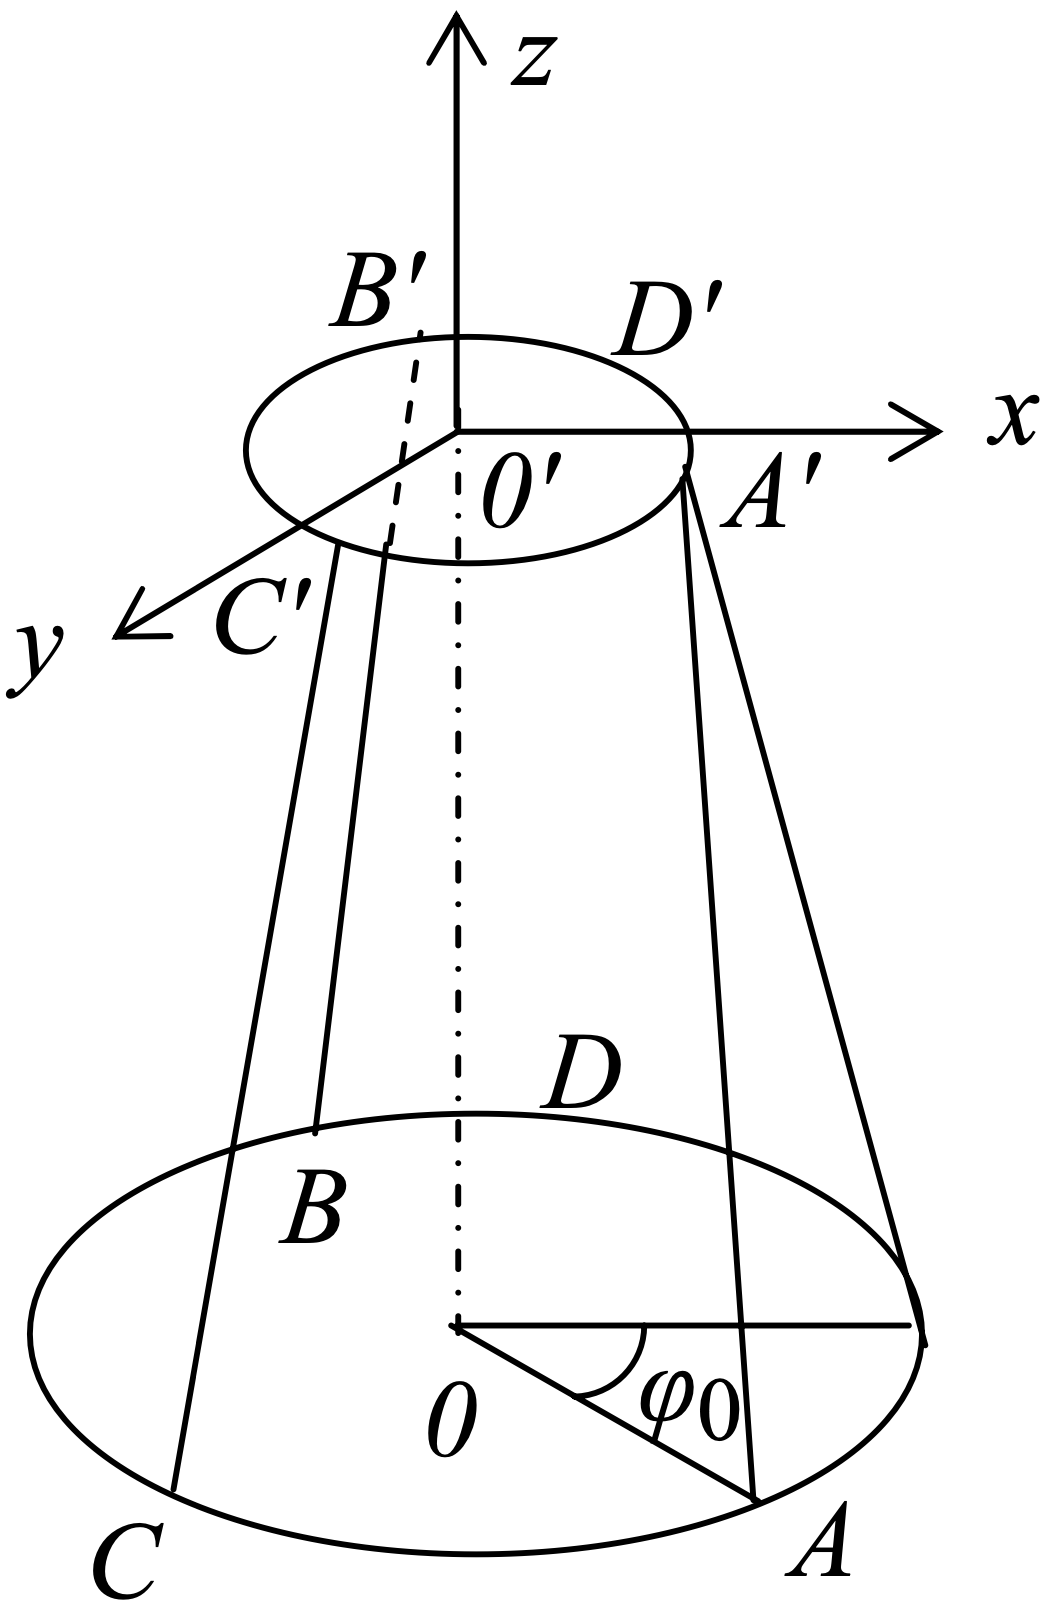
\includegraphics[width=0.3\textwidth]{pictures/PictureOne}
		\caption{Трифилярный подвес}\label{PicOne}
	\end{center}
\end{figure}
На рисунке~\ref{PicOne} изображён трифилярный подвес. Он состоит из подвижной круглой платформы $D$ радиуса $R$, подвешенной к платформе $D'$ радиуса $r<R$ на трех симметрично расположенных нитях $AA'$, $BB'$, $CC'$ длинами $l$. Платформа может совершать крутильные колебания вокруг вертикальной оси $OO'$. Центр тяжести при этом перемещается вертикально по оси вращения.